\documentclass[10pt]{article}
\usepackage[pdftex]{graphicx}
\usepackage{subcaption}
\graphicspath{{./images/}}
\usepackage{amsmath,amssymb}
\usepackage{dirtytalk}
\usepackage{anyfontsize}
\usepackage{xcolor}
\usepackage{hyperref}
\usepackage{graphicx} 
\usepackage{placeins}
\hypersetup{
	colorlinks,
	linkcolor={red!50!black},
	citecolor={blue!50!black},
	urlcolor={blue!80!black}
}
\usepackage[skip=10pt plus1pt, indent=40pt]{parskip}
\usepackage{../common-styles/csagh}


\begin{document}
	\begin{opening}
		\title{Avance - PIA Investigación de Operaciones}
		\author[Universidad Autónoma de Nuevo León, San Nicolás de los Garza, aldo.hernandezt@uanl.edu.mx]{Aldo Hernández}
		\author[Universidad Autónoma de Nuevo León, San Nicolás de los Garza, abraham.lopezg@uanl.edu.mx]{Abraham López}
		
		\begin{abstract}
            El Instituto Mexicano del Seguro Social es la entidad más popular y accesible para recibir atención médica a nivel nacional, sin embargo es debido a esta misma razón que es común una gran cantidad de pacientes diarios en cada una de las unidades médicas, lo que alarga los tiempos de atención para todos los ciudadanos que requieren algún tipo de procedimiento médico. Este estudio busca encontrar los tiempos de espera promedio para los pacientes y la cantidad de servidores necesarios para convertir el sistema en uno estable con el propósito de ofrecer alternativas para una mejor calidad de atención al paciente. Para lograr esto, se utilizará la teoría de colas para modelar un sistema particular en serie (o también conocido como tándem) y encontrar las medidas de desempeño para su posterior análisis. El estudio indicó a partir de datos y algunas suposiciones que en un caso general de un paciente referido entre dos unidades médicas es inestable y por consecuencia ineficiente, además las soluciones propuestas son aumentar la cantidad de servidores en cada unidad y cambiar la disciplina de las colas.
		\end{abstract}

		\keywords{colas, IMSS, python}
	\end{opening}
	
	\section{Introducción}
	La teoría de colas es una rama de las matemáticas que estudia el comportamiento de líneas de espera, buscando optimizar la eficiencia en los sistemas de servicio, en ella se analizan elementos como las tasas de llegada de usuarios, las tasas de servicio, el número de servidores y el orden de atención, entre otros factores. Este estudio se basa en un sistema de colas en serie (o tándem), donde distintos flujos de pacientes deben ser canalizados hacia un único punto de atención especializado, también conocido como un sistema de colas de múltiples entradas y una sola salida.
	
    Dentro del sistema de salud, la capacidad hospitalaria de una unidad médica se enfoca en atender las necesidades de los pacientes a través de la organización \cite{MEDESK}, funcionamiento, gestión del personal, así como de la funcionalidad y disponibilidad de los recursos físicos y tecnológicos con los que debe contar un establecimiento de salud, calculados en función a sus características, dotación de recursos y demanda de atención. Algunos de los problemas más importantes que enfrentan estas unidades son su baja capacidad, las demoras y la programación inadecuada de sus recursos \cite{MEDESK} y podemos notar que estos tres problemas están relacionados, por ejemplo, una programación inadecuada de los pocos recursos y personal conlleva mayores tiempos de atención (e incluso servicio) por paciente.
    
    Es importante mencionar que la falta de recursos no suele ser un problema que dependa de la unidad completamente, sino que se ve influenciado por la fracción del presupuesto anual que destine el gobierno al sector de salud pública. Sin embargo, es común que la mala organización de dichos recursos acentúe esta falta de presupuesto más de lo que es; aquí es donde surge el problema de la optimización en la administración de estos recursos con el fin de lograr una mayor capacidad de servicio con un menor costo para la unidad.
    
    Por otra parte, además de la capacidad resolutiva de cada unidad, es fundamental diferenciar a las unidades en niveles de atención. Esto permite establecer un flujo de atención organizado y armonizado para las personas cuyas atenciones requieren transitar en tres diferentes niveles, con el fin de evitar la acumulación de pacientes en las distintas unidades de salud y lograr un menor tiempo de servicio.
    
    Para establecer de forma adecuada la vinculación de los tres niveles de atención, se requiere primeramente identificar el total de unidades médicas en operación dentro del sistema de salud y clasificarlas por nivel de atención de acuerdo a sus recursos, personal y cartera de servicios.
    
    A pesar de este sistema de tres fases o niveles, la demanda de servicios de salud por unidad sigue siendo bastante alta, sobretodo en el primer nivel ya que no es necesario hacer cita previa para tener una consulta. Para evidenciar esto solo basta con acudir a cualquier unidad del seguro social para recibir una consulta, es tanta la reputación que tiene esta organización sobre la calidad de servicio y tiempo de espera que podría preguntarle a cualquier persona registrada en el seguro social si ha tenido alguna mala experiencia con estos temas. Es por esto que el IMSS ideó un sistema llamado UNIFILA a principios de 2017 para estos casos \cite{UNIFILA}, esta idea ofrece tres opciones para los pacientes sin cita:
    \begin{enumerate}
    	\item Programar el mismo día una cita con su médico familiar.
    	\item Programar una cita con su médico familiar la fecha más próxima.
    	\item Pasar al módulo UNIFILA para obtener una cita en los consultorios con espacios disponibles.
    \end{enumerate}
    
    Si bien esta implementación es bastante prometedora teóricamente, en la práctica resulta contraproducente ya que los testimonios de tiempos de espera siguen siendo bastante altos; esto podría ser debido a que si una gran sección de los pacientes ingresan a una clínica sin cita pues a final de cuentas todos tendrían que esperar a que se liberen espacios en los consultorios que estén ocupados por las personas que ya tienen cita.
    
    El problema que abordaremos se centra en el seguimiento de pacientes del primer nivel de atención hacia el tercer nivel dentro del sistema de salud del IMSS (Instituto Mexicano del Seguro Social), para ello, utilizaremos dos conjuntos de datos de consultas: uno sobre unidades de primer nivel y otro sobre las de tercer nivel. Estos datos contienen información de atenciones médicas realizadas en septiembre de 2017 mediante la encuesta EnSat \cite{ensat2017} llevada a cabo al menos una vez al año por el IMSS.
    
    Se eligieron los resultados de este año ya que es uno de los conjuntos con más registros de información y también debido a que a partir de 2019 se sustituyó esta encuesta por otra llamada EnCal; si bien esta encuesta está mejor estructurada, también omite muchas preguntas relevantes para este estudio.
    
    El principal enfoque para el estudio serán los tiempos de espera basándonos en la siguiente pregunta: ¿por qué el paciente promedio tiene que esperar tantos días para recibir la atención médica que necesita?

	\section{Contexto} \label{sec:contexto}
	En el sistema de salud del IMSS, los pacientes deben ser atendidos inicialmente en unidades médicas de primer nivel, éstas otorgan exclusivamente atención ambulatoria, que puede ser general o especializada; en dichas unidades inicia el primer contacto con los pacientes fungiendo como principales vehículos para realizar acciones de prevención y promoción a la salud, así como la detección temprana y seguimiento de enfermedades, son la vía de entrada al sistema de atención y, en caso necesario, son referidos a hospitales de tercer nivel, que son las que otorgan atención médica hospitalaria para la atención de padecimientos de alta especialidad y de urgencias.
	
    Este proyecto se centrará específicamente en la Unidad Médica Familiar No. 28 (UMF 28) de Monterrey, Nuevo León, como punto de primer nivel, y en el Hospital de Especialidades No. 25 de Monterrey como punto de tercer nivel, ambos centros de atención se encuentran geográficamente cercanos, lo cual facilita el análisis de la transferencia de pacientes entre ellos.
    
    \begin{figure}[h]
		\centering
		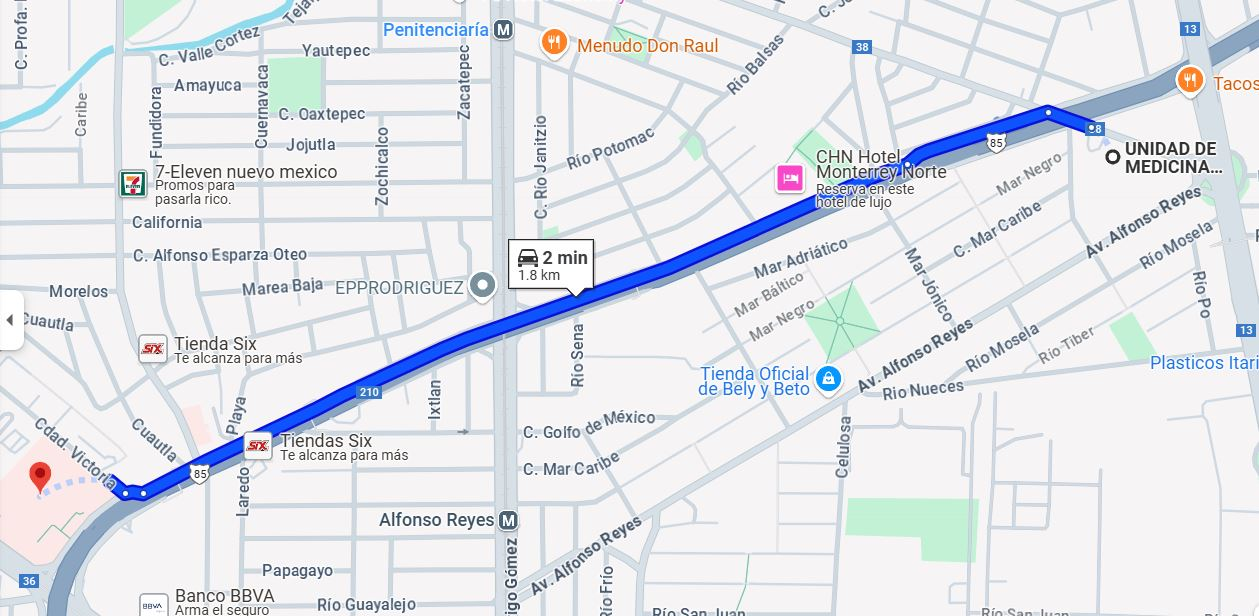
\includegraphics[width=90mm]{./images/mapa.jpg}
		\caption{Distancia entre los dos centros.}
	\end{figure}
	\FloatBarrier

    Antes de proceder con el análisis, será necesario realizar un proceso de limpieza de los conjuntos de datos, pues decidimos que no haremos distinciones en cuestión de edades, sexo o tipo de paciente aunque existan columnas que nos hablen sobre estas características de la persona, por lo que eliminaremos los registros no necesarios y seleccionaremos solo aquellos campos relevantes para el propósito de este estudio como lo son los tiempos de espera y el servicio otorgado.
    
    El flujo de atención será modelado en tres etapas:

    \begin{enumerate}
        \item \textbf{Primera etapa (UMF 28)}: Los pacientes llegan a consulta general, donde son atendidos por múltiples médicos de primer contacto. Esta situación se modela mediante un sistema de colas \textbf{M/M/s}.
        
        \item \textbf{Segunda etapa (Proceso de referencia)}: Los pacientes que requieren atención especializada son referidos a través de un proceso administrativo, modelado como un sistema de colas \textbf{M/M/1}.
        
        \item \textbf{Tercera etapa (Hospital 25)}: Los pacientes son atendidos por múltiples especialistas de tercer nivel, modelado nuevamente como un sistema de colas \textbf{M/M/s}.
    \end{enumerate}

    \begin{figure}[h]
		\centering
		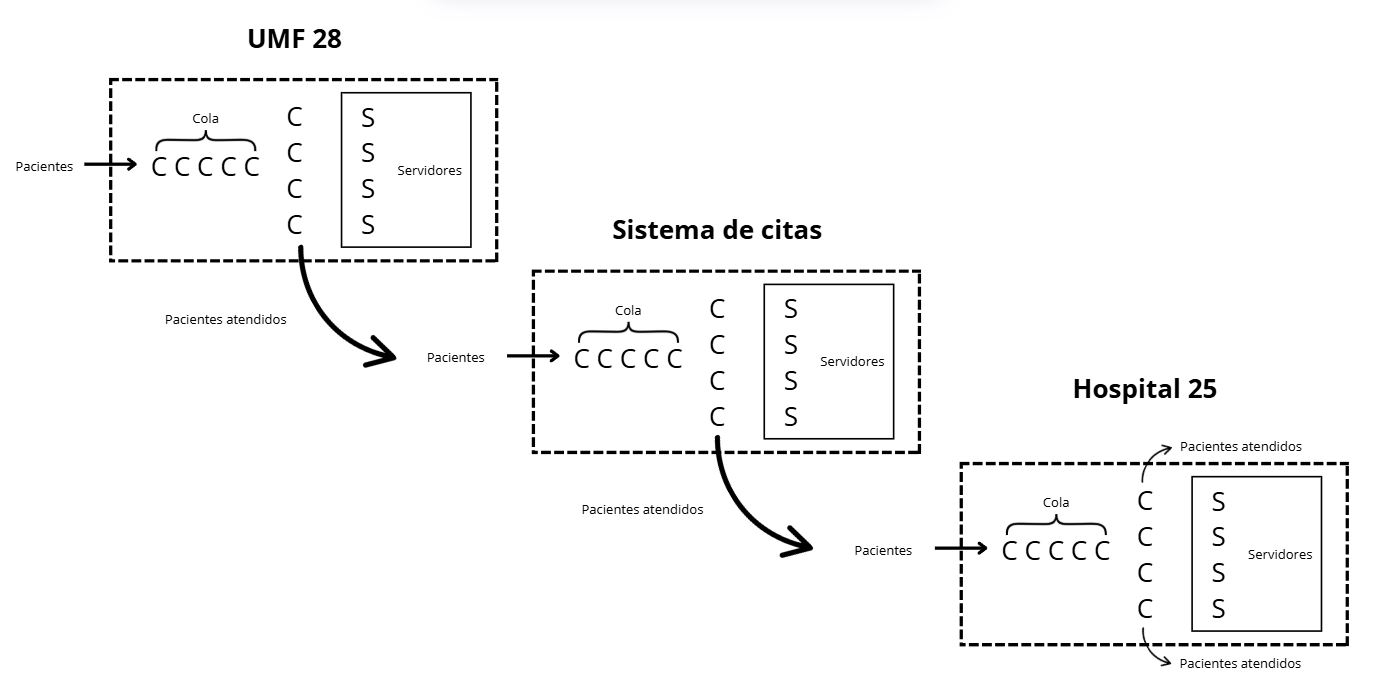
\includegraphics[width=130mm]{./images/sistema.jpg}
		\caption{Modelo.}
	\end{figure}

    Una vez que el paciente recibe la atención especializada, existen tres posibles desenlaces, el paciente se cura y no requiere más atención (salida del sistema), el paciente requiere seguimiento y debe regresar al hospital o el paciente abandona el tratamiento por voluntad propia. Cabe aclarar que este estudio se concentrará en el caso de la salida del sistema, puesto que asumimos un caso ideal en el que el paciente busca mejorarse y además no tiene múltiples consultas ya que eso agrandaría el flujo del sistema a estudiar.

    \section{Datos y problema}
    Después de realizar una limpieza básica para eliminar datos innecesarios y registros vacíos, filtramos únicamente los datos correspondientes a las unidades médicas mencionadas. Además, es importante mencionar que se asumió una distribución de probabilidad exponencial para cada una de las colas tanto para los tiempos entre llegadas como los tiempos de servicio. En las siguientes subsecciones se explicarán los procesos llevados a cabo en cada una de las colas.
    
    El caso general a estudiar se detallará a continuación. Una persona con seguro social en el IMSS comienza a tener síntomas de alguna enfermedad, por lo que acude a la Unidad de Medicina Familiar 28 para una consulta de primer nivel. Al llegar al centro de salud, tiene que esperar en una sala mientras se libera un consultorio para que lo puedan atender y cuando finalmente lo revisa el doctor en turno, resulta que su caso requiere de un chequeo realizado por un especialista, por lo que es referenciado al Hospital de Especialidades 25. Sin embargo, el paciente tiene que sacar una cita previa para poder ser recibido en el hospital para consulta, por lo que al tramitarla la espera es de varios días. Finalmente, acude el día de su cita al centro de salud donde todavía tiene que volver a esperar en una sala para que lo pasen a un consultorio, una vez saliendo del chequeo, el paciente empieza su tratamiento y eventualmente se le da de alta.
    
    Es importante mencionar que este caso no es tan común y que se hacen varias suposiciones a lo largo del estudio, como que todos los pacientes que salen de la UMF y son referidos a otra instalación, es directamente al Hospital de Especialidades, cuando es claro que no todos los casos son así. Sin embargo, esto nos sirve como una buena aproximación para los casos reales.
    
    \subsection{Primera cola (M/M/$s_{1}$)}
    Los pacientes se generan en una fuente de entrada finita lo suficientemente grande como para no preocuparnos por la población debido a que este tipo de unidades casi nunca se saturan de pacientes, por lo que se tomará como una fuente ilimitada. Además, se asumirá una distribución Poisson para las llegadas de pacientes bajo el supuesto de que llegan aleatoriamente con una cierta tasa media fija, por lo que el tiempo entre llegadas sigue una distribución exponencial. Se ignorarán los casos en los que los pacientes se rehúsan a entrar al sistema (debido a que en un caso ideal su salud debería ser la prioridad) junto con la distinción de grupos entre los pacientes (por edad, enfermedad, entre otros) de tal manera que para cálculos generales se considerará el conjunto completo mientras que para las medidas de desempeño solo se tomarán en cuenta datos de pacientes del caso general del sistema de colas.
    
    La cola se considerará infinita a pesar de tener alguna cota superior ya que tomarla en cuenta complicaría el análisis. Esta cola tendrá una disciplina FCFS, de manera que los pacientes serán atendidos a como vayan llegando a la sala de espera.
    
    La estación de servicio contiene $s_{1}$ servidores activos la jornada completa de 12 horas cuyos tiempos de servicio siguen una distribución exponencial para todos los pacientes. Nótese que $s_{1}$ todavía no está definida, por lo que estudiaremos distintos valores para dicha variable a fin de encontrar un balance entre costos y tiempos de espera.
    
    Finalmente, medimos los siguientes parámetros para esta cola:
    
    \begin{equation*}
    	\left\{
    		\begin{array}{@{}l@{}}
	    		\frac{1}{\lambda} = \frac{720 \text{ minutos}}{1599 \text{ pacientes}} = 0.45 \text{ minutos por paciente,} \\
	    		\lambda = 2.22 \text{ pacientes llegan en promedio por minuto,} \\
	    		\frac{1}{\mu} = 15 \text{ minutos por paciente,} \\
	    		\mu = 0.066 \text{ pacientes por minuto atendidos en promedio,} \\
	    		W_{q} = 18.64 \text{ minutos en promedio en la cola,} \\
	    		W = 33.64 \text{ minutos en promedio en el sistema,} \\
	    		\left\lceil L \right\rceil = 75 \text{ pacientes en promedio en el sistema,} \\
	    		\left\lfloor L_{q} \right\rfloor = 41 \text{ pacientes en promedio en la cola}
    		\end{array}
   		\right.\,.
    \end{equation*}
    
    Para obtener esta información bastó con revisar la información del conjunto de datos \cite{ensat2017} para conocer los pacientes diarios en promedio en la UMF 28 Monterrey en 2016 y asumir un tiempo de servicio de 15 minutos. Además, se consultó el conjunto de datos \cite{ensat2017} para obtener el tiempo de espera promedio en la cola mediante una media de datos agrupados según los datos que se muestran en la figura \ref{fig:frec_espera_umf28}. Para los valores de $L$ y $L_{q}$ se optó por usar la función piso o techo según si los decimales eran despreciables o no, respectivamente, ya que tienen que ser números enteros.
    
    Además, podemos deducir a partir de $L$ y $L_{q}$ que hay en promedio 34 pacientes atendidos, lo que indica que para que el sistema sea estable entonces $s_{1} \geq 34$. Esto también se demuestra con la siguiente desigualdad
    
    \begin{equation*}
    	\rho = \frac{\lambda}{s_{1}\mu} = \frac{2.22}{s_{1}(0.066)} < 1
    	\therefore s_{1} > 33.64
    \end{equation*}
    
    \begin{figure}[h]
    	\centering
    	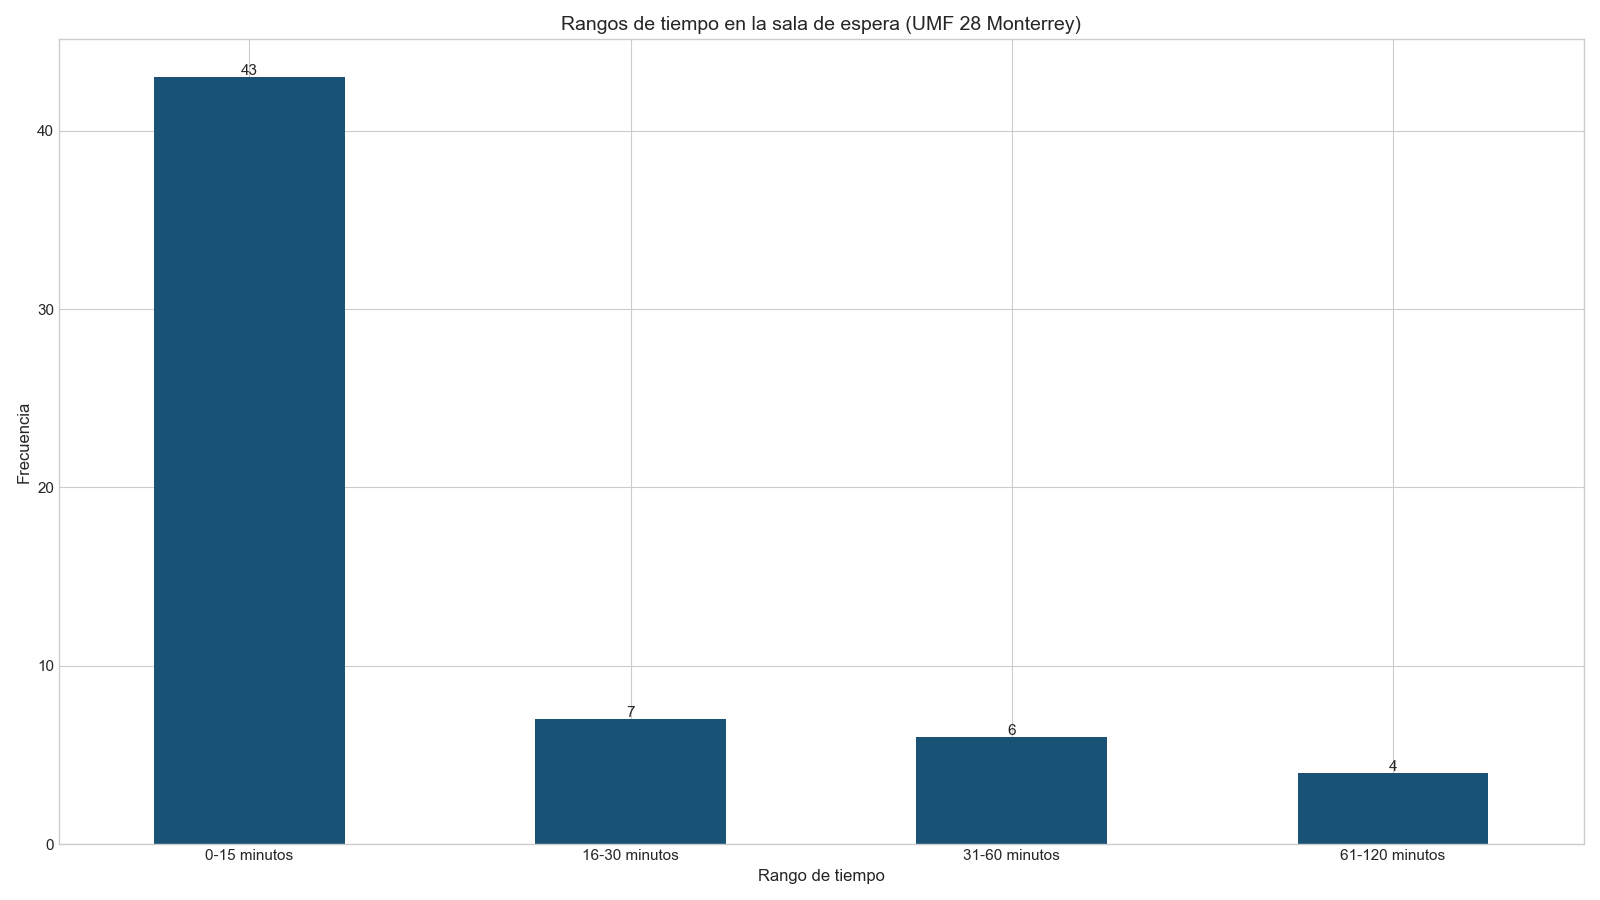
\includegraphics[width=\linewidth]{./images/rangos-tiempo-espera-umf28.png}
    	\caption{Gráfica de frecuencias para los tiempos de espera en la UMF 28.}
    	\label{fig:frec_espera_umf28}
    \end{figure}
    
    \newpage
    
    \subsection{Segunda cola (M/M/1)}
    Los pacientes se generan en una fuente de entrada finita lo suficientemente grande como para no preocuparnos por la población debido a que en el flujo del sistema estos pacientes son aquellos que al salir de su consulta en alguna unidad de primer nivel de atención requieren una cita posterior en una unidad de tercer nivel, entonces se tomará como una fuente ilimitada. Además, se asumirá una distribución Poisson para las llegadas de pacientes bajo el supuesto de que llegan aleatoriamente con una cierta tasa media fija, por lo que el tiempo entre llegadas sigue una distribución exponencial. Se ignorarán los casos en los que los pacientes se rehúsan a entrar al sistema (debido a que en un caso ideal su salud debería ser la prioridad) junto con la distinción de grupos entre los pacientes (por edad, enfermedad, entre otros).
    
    La cola se considerará infinita a pesar de tener alguna cota superior ya que tomarla en cuenta complicaría el análisis. Esta cola tendrá una disciplina FCFS, de manera que los pacientes serán atendidos a como vayan solicitando su cita en el IMSS.
    
    La estación de servicio contiene un único servidor activo (el "sistema") las 24 horas del día y sus tiempos de servicio siguen una distribución exponencial para todos los pacientes.
    
    Finalmente, medimos los siguientes parámetros para esta cola:
    
    \newpage
    
    \begin{equation*}
    	\left\{
    	\begin{array}{@{}l@{}}
    		\frac{1}{\lambda} = \frac{1 \text{ día}}{734880 \text{ pacientes}} = 0.00000136076 \text{ días por paciente (casi 9 pacientes por segundo),} \\
    		\lambda = 734880 \text{ pacientes llegan en promedio por día,} \\
    		\frac{1}{\mu} = 0.00000136076 \text{ día por paciente,} \\
    		\mu = 734880 \text{ pacientes por día atendidos en promedio,} \\
    		W_{q} = 17.51999 \text{ días en promedio en la cola,} \\
    		W = 17.52 \text{ días en promedio en el sistema,} \\
    		\left\lceil L \right\rceil = 12,875,098 \text{ pacientes en promedio en el sistema,} \\
    		\left\lceil L_{q} \right\rceil = 12,875,097 \text{ pacientes en promedio en la cola}
    	\end{array}
    	\right.\,.
    \end{equation*}
    
    Para obtener esta información se consultó el conjunto de datos para obtener el tiempo de espera promedio en la cola mediante una media de datos agrupados según los datos que se muestran en la figura \ref{fig:frec_espera_cita}. También, se asumió el valor de $\frac{1}{\lambda}$ de manera que son $4 \frac{\text{pacientes}}{\text{hora}} \times 12 \frac{\text{horas de jornada}}{\text{día}} \times 10 \frac{\text{servidores promedio}}{\text{UMF}} \times 1531 \text{ UMF} = 734880 \text{ pacientes.}$
    
    \begin{figure}[h]
    	\centering
    	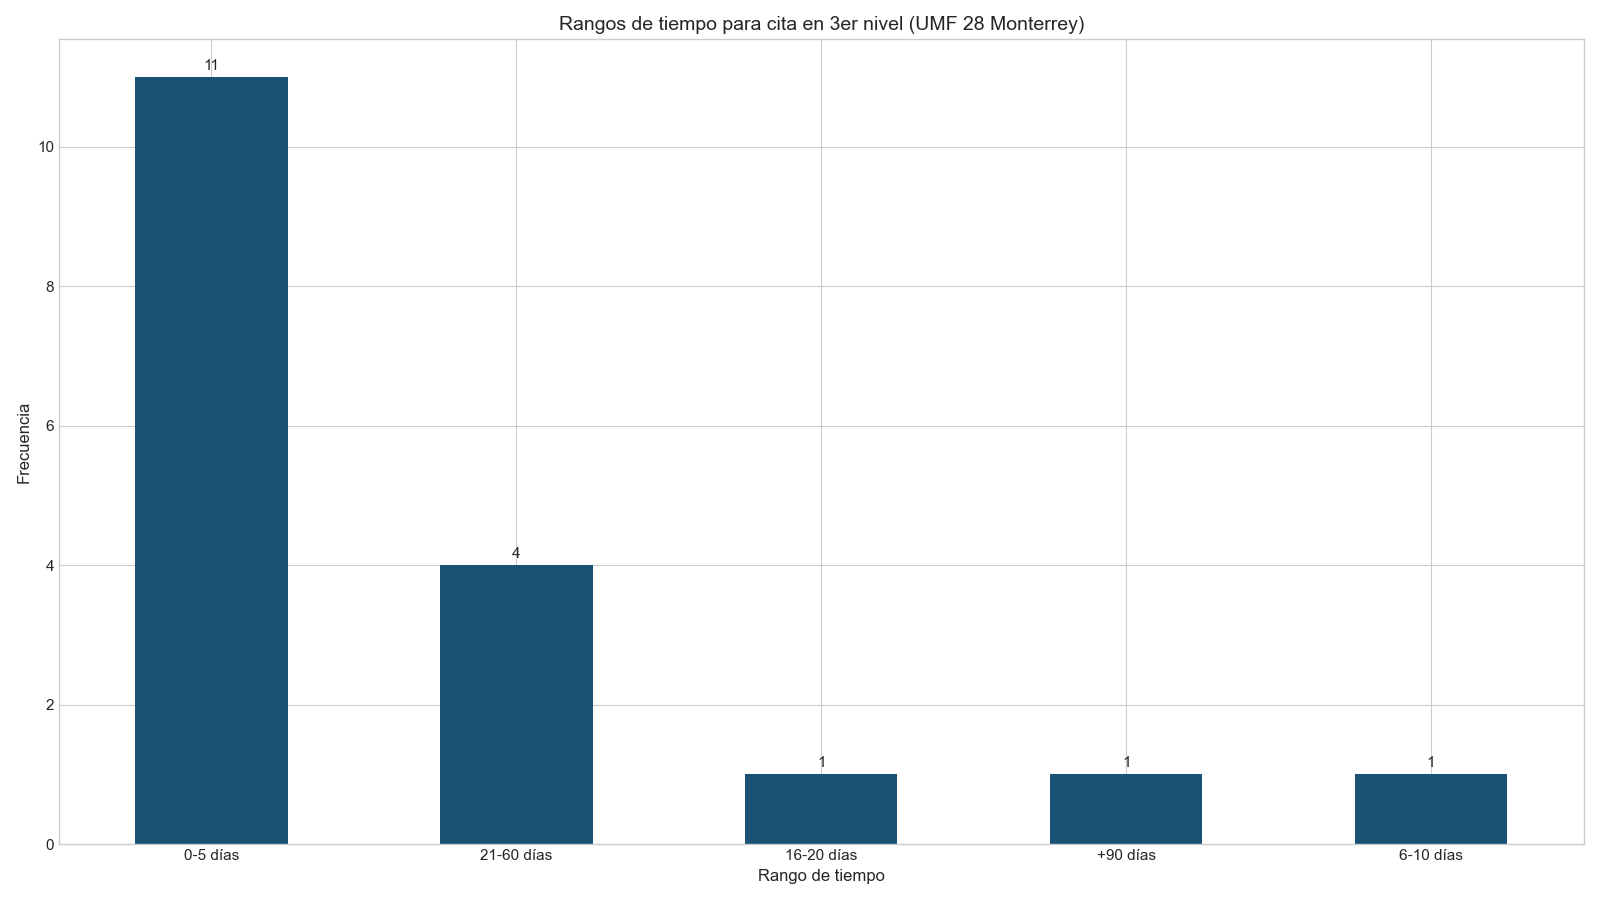
\includegraphics[width=\linewidth]{./images/rangos-tiempo-3-umf28.png}
    	\caption{Gráfica de frecuencias para los tiempos de espera en el sistema de citas.}
    	\label{fig:frec_espera_cita}
    \end{figure}
    
    \subsection{Tercera cola (M/M/$s_{2}$)}
    Los pacientes se generan en una fuente de entrada finita lo suficientemente grande como para no preocuparnos por la población debido a que este tipo de unidades de alta especialidad casi nunca se saturan de pacientes, entonces se tomará como una fuente ilimitada. Además, se asumirá una distribución Poisson para las llegadas de pacientes bajo el supuesto de que llegan aleatoriamente con una cierta tasa media fija dictada por el sistema de citas, por lo que el tiempo entre llegadas sigue una distribución exponencial. Se ignorarán los casos en los que los pacientes se rehúsan a entrar al sistema (debido a que en un caso ideal su salud debería ser la prioridad) junto con la distinción de grupos entre los pacientes (por edad, enfermedad, entre otros).
    
    La cola se considerará infinita a pesar de tener alguna cota superior ya que tomarla en cuenta complicaría el análisis. Esta cola tendrá una disciplina FCFS, de manera que los pacientes serán atendidos a como vayan llegando a la sala de espera.
    
    La estación de servicio contiene $s_{2}$ servidores activos la jornada completa de 12 horas cuyos tiempos de servicio siguen una distribución exponencial para todos los pacientes. Nótese que $s_{2}$ todavía no está definida, por lo que estudiaremos distintos valores para dicha variable a fin de encontrar un balance entre costos y tiempos de espera.
    
    Finalmente, medimos los siguientes parámetros para esta cola: 
    
    \begin{equation*}
    	\left\{
    	\begin{array}{@{}l@{}}
    		\frac{1}{\lambda} = \frac{720 \text{ minutos}}{715 \text{ pacientes}} = 1.01 \text{ minutos por paciente,} \\
    		\lambda = 0.99 \text{ pacientes llegan en promedio por minuto,} \\
    		\frac{1}{\mu} = 30 \text{ minutos por paciente,} \\
    		\mu = 0.033 \text{ pacientes por minuto atendidos en promedio,} \\
    		W_{q} = 18.51 \text{ minutos en promedio en la cola,} \\
    		W = 48.51 \text{ minutos en promedio en el sistema,} \\
    		\left\lceil L \right\rceil = 49 \text{ pacientes en promedio en el sistema,} \\
    		\left\lfloor L_{q} \right\rfloor = 18 \text{ pacientes en promedio en la cola}
    	\end{array}
    	\right.\,.
    \end{equation*}
    
    Para obtener esta información bastó con revisar el conjunto de datos para obtener dos cosas principalmente: el tiempo de espera promedio en la cola mediante una media de datos agrupados según los datos que se muestran en la figura \ref{fig:frec_espera_hes25} y los pacientes diarios que acuden con un especialista en 2016. Por otro lado, para los valores de $L$ y $L_{q}$ se optó por usar la función piso o techo según si los decimales eran despreciables o no, respectivamente, ya que tienen que ser números enteros.
    
    Igual que en la primera cola, a partir de $L$ y $L_{q}$ podemos deducir que $s_{2} \geq 31$ para que el sistema sea estable y que se cumpla la siguiente desigualdad
    
    \begin{equation*}
    	\rho = \frac{\lambda}{s_{2}\mu} = \frac{0.99}{(31)(0.033)} < 1
    \end{equation*}
    
    \begin{figure}[h]
    	\centering
    	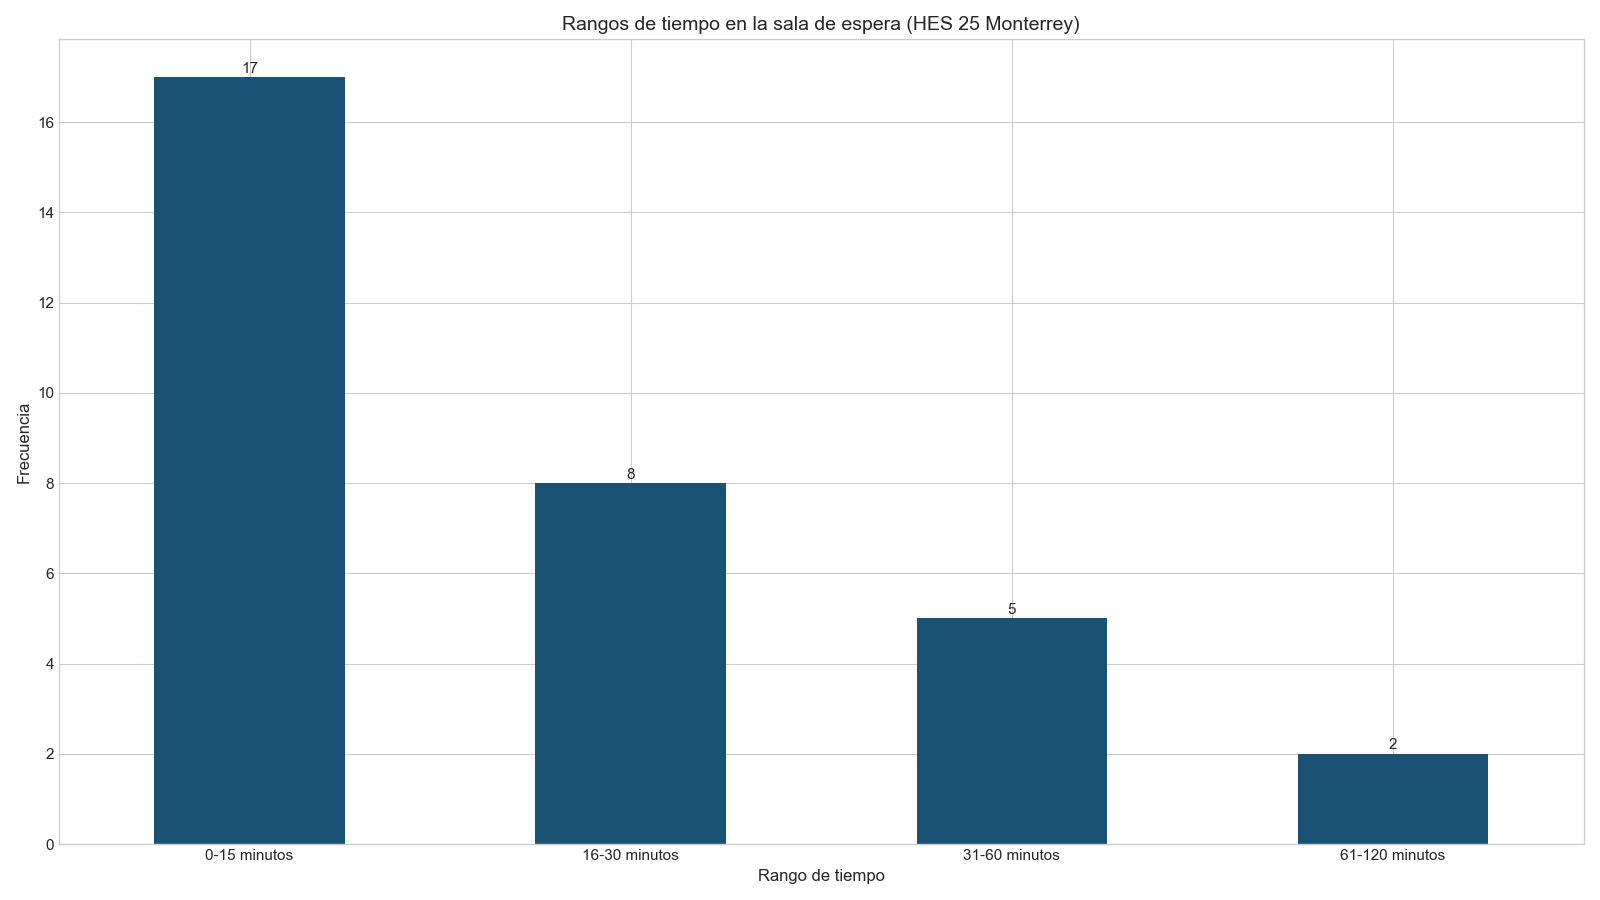
\includegraphics[width=130mm]{./images/rangos-tiempo-espera-hes25.png}
    	\caption{Gráfica de frecuencias para los tiempos de espera en el HES 25.}
    	\label{fig:frec_espera_hes25}
    \end{figure}
    
    \newpage
    
    \section{Desarrollo} \label{sec:desarrollo}
    \subsection{Cola de espera en UMF 28}
    Como se había mencionado con anterioridad, para que esta línea de espera sea estable se requiere que existan al menos 34 consultorios en la Unidad de Medicina Familiar 28. Si bien no es posible saber el número de servidores exactos debido a la falta de información, podemos dividir el análisis en dos partes: una cola estable y otra inestable.
    
    \subsubsection{Cola estable}
    Tomando en cuenta $s_{1} = 34$ entonces $\rho$ está muy cercano a uno, lo que significa que esencialmente la cola siempre estará saturada, es decir, las colas siempre serán largas y los servidores estarán en constante trabajo. Esto es malo por diversas razones, pero principalmente hay dos: las personas que requieren atención médica tendrán que esperar 18 minutos en promedio para ser atendidos y los médicos generales estarán dando consultas continuas, por lo que es normal pensar que habría que dividir las jornadas de trabajo entre todo el personal médico, incurriendo en más gastos para la unidad médica al tener que pagar más o mayores sueldos. 
    
    Viendo estos problemas, es fácil pensar que si se aumenta el número de consultorios, se eliminaría al menos uno de estos problemas en gran escala. Consultando la figura \ref{fig:valores_s1} es evidente que para un mismo $\rho$ el sistema con menos servidores ($34$) gestiona mejor las colas ya que tiene colas más cortas, sin embargo estas mediciones son relativas a la carga de trabajo. Tomando en cuenta los distintos valores de $s_{1}$ mostrados en la gráfica, calculamos $\rho$:
    
    \begin{equation*}
    	\left\{
    	\begin{array}{@{}l@{}}
    		\rho_{1} = \frac{2.22}{(34)(0.066)} \approx 0.989 ; L_{1} \approx 120 \\
    		\rho_{2} = \frac{2.22}{(50)(0.066)} \approx 0.673 ; L_{2} \approx 34 \\
    		\rho_{3} = \frac{2.22}{(70)(0.066)} \approx 0.481 ; L_{3} \approx 34 \\
    		\rho_{4} = \frac{2.22}{(100)(0.066)} \approx 0.336 ; L_{4} \approx 34 \\
    		\rho_{5} = \frac{2.22}{(140)(0.066)} \approx 0.240 ; L_{5} \approx 34 \\
    	\end{array}
    	\right.\,.
    \end{equation*}
    
    \begin{figure}[!ht]
    	\centering
    	
    	\begin{subfigure}[c]{0.65\textwidth}
    		\centering
    		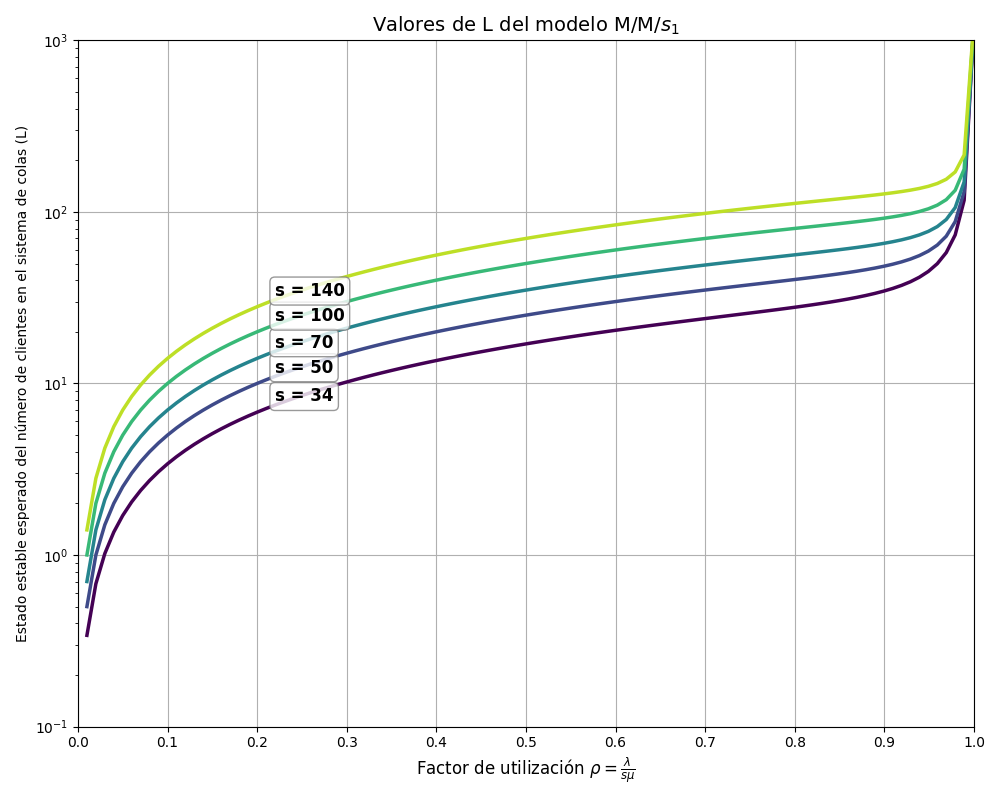
\includegraphics[width=\textwidth]{./images/rho-l-s1.png}
    		\caption{Valores de $L$ para distintos servidores.}
    		\label{fig:valores_s1}
    	\end{subfigure}
    	\begin{subfigure}[c]{0.3\textwidth}
    		\centering
    		\label{s1_comp}
    		\begin{tabular}{|c|c|c|}
    			\hline
    			$s_{1}$ & $\rho$ & $L$ \\
    			\hline
    			34 & 0.989 & 119.377 \\
    			35 & 0.961 & 52.053 \\
    			36 & 0.934 & 42.095 \\
    			37 & 0.909 & 38.311 \\
    			40 & 0.841 & 34.746 \\
    			45 & 0.747 & 33.758 \\
    			50 & 0.673 & 33.648 \\
    			70 & 0.481 & 33.636 \\
    			100 & 0.336 & 33.636 \\
    			140 & 0.240 & 33.636 \\
    			\hline
    		\end{tabular}
    		\caption{Convergencia de $L$.}
    		\label{tab:s1_comp}
    	\end{subfigure}
    	\caption{Relación entre valores de $L$ y parámetros de la primera cola.}
    	\label{fig:analisis_s1}
    \end{figure}
    
    A pesar de que una cola con menos servidores es más eficiente bajo una carga relativa de trabajo igual, al aumentar el número de servidores en la cola podríamos reducir la cantidad de pacientes en espera. Aún más, podemos notar en la tabla \ref{s1_comp} que a mayor valor de $s_{1}$, $L$ se aproxima más a 34, lo que quiere decir que no habría ninguna línea de espera; de hecho, este valor converge rápidamente y para un aumento de un solo consultorio se estaría reduciendo la cantidad de personas en la cola en menos de la mitad.
    
    \subsubsection{Cola inestable} \label{sssec:inestable1}
    Si consideramos $s_{1} \leq 33$, entonces esta cola estaría siempre saturada operando bajo una sobrecarga de pacientes, ocasionando que no todos sean atendidos y que los servidores nunca dejen de trabajar. Esto sería un problema bastante grave ya que la cola crecerá indefinidamente con el tiempo hasta que dejen de ofrecer servicio en la unidad médica (por los horarios de atención) y los tiempos de espera aumentarán durante el transcurso del día, generando disconformidad en los pacientes.
    
    \subsection{Cola de espera en sistema de citas}
    Para la segunda cola en el sistema, podemos asumir que se trata de una cola estable pero extremadamente saturada. Esto explicaría los grandes tiempos de espera para poder acudir con cita al hospital que se desea. Además, todos los pacientes en la cola en algún tiempo serán atendidos eventualmente debido a que asumimos que el "sistema" nunca descansa y siempre se están asignando citas.
    
    En este caso, es irrelevante hacer cálculos para $\rho$ debido a lo ya mencionado y a que al ser un sistema nacional, es normal que esté sobrecargado ya que la única manera de agilizar este procedimiento sería construyendo más centros de salud según el crecimiento de la fuente de entrada.
    
    \subsection{Cola de espera en HES 25}
    Para que esta cola sea estable se requiere que existan al menos 31 consultorios en Hospital de Especialidades 25. Al no poder saber el número de servidores reales, el análisis se dividirá en dos partes como en la primera cola: una estable y otra inestable.
    
    \subsubsection{Cola estable}
    Al igual que en la primera línea de espera, cuando $s_{2} = 31$ entonces $\rho$ está muy cerca del 1, indicando una gran carga de trabajo para el sistema. Aquí, los pacientes tienen que esperar en promedio 18 minutos antes de ser atendidos por un especialista; además, al tratarse de médicos especialistas, el sueldo que se tiene que pagar es mayor, generando más gastos para la unidad médica.
    
    Observamos en la figura \ref{fig:valores_s2} que un sistema con menos servidores es más eficiente relativamente bajo un mismo valor de $\rho$; pero si aumentamos el número de servidores, $\rho$ disminuye considerablemente rápido según la tabla \ref{tab:s2_comp}. Además, con un aumento de $4$ consultorios estaríamos prácticamente eliminando las colas de espera.
    
    \begin{figure}[!ht]
    	\centering
    	
    	\begin{subfigure}[c]{0.65\textwidth}
    		\centering
    		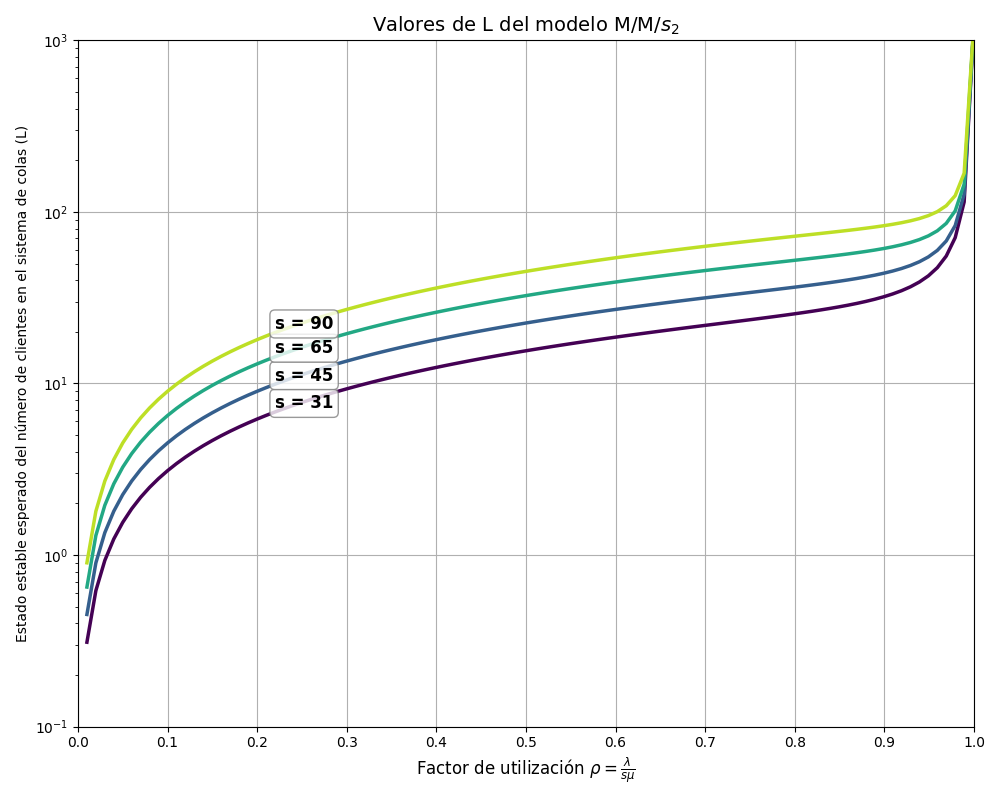
\includegraphics[width=\textwidth]{./images/rho-l-s2.png}
    		\caption{Valores de $L$ para distintos servidores.}
    		\label{fig:valores_s2}
    	\end{subfigure}
    	\begin{subfigure}[c]{0.3\textwidth}
    		\centering
    		\begin{tabular}{|c|c|c|}
    			\hline
    			$s_{2}$ & $\rho$ & $L$ \\
    			\hline
    			31 & 0.968 & 53.968 \\
    			32 & 0.938 & 39.453 \\
    			33 & 0.909 & 34.905 \\
    			34 & 0.882 & 32.823 \\
    			35 & 0.857 & 31.707 \\
    			45 & 0.667 & 30.014 \\
    			65 & 0.462 & 30.000 \\
    			90 & 0.333 & 30.000 \\
    			140 & 0.214 & 30.000 \\
    			\hline
    		\end{tabular}
    		\caption{Convergencia de $L$.}
    		\label{tab:s2_comp}
    	\end{subfigure}
    	\caption{Relación entre valores de $L$ y parámetros de la tercera cola.}
    	\label{fig:analisis_s2}
    \end{figure}
    
    \subsubsection{Cola inestable}
    Tomando en cuenta $s_{1} \leq 30$, la cola estaría siempre bajo una carga excesiva de pacientes, ocasionando que no todos sean atendidos y que los médicos que ofrecen consultas nunca dejen de trabajar. Esto además de generar los mismos problemas que el caso visto en el apartado \ref{sssec:inestable1} del documento, sería todavía más grave ya que los pacientes que acuden a las unidades médicas de tercer nivel por lo general requieren seguimiento médico lo antes posible.
    
    \newpage
    
    \subsection{Sistema en serie}
    En general, podemos decir que en promedio un paciente que se adapta a nuestro caso general explicado en la sección \ref{sec:contexto} dura aproximadamente 17 días con 13 horas en el sistema: 17 días con 12 horas en recibir una cita para el HES 25 y cerca de 1 hora esperando en filas.
    
    Desde el punto de vista del paciente esta cantidad excesiva de tiempos de espera no es ideal, aunque es hasta cierto punto normal por la cantidad de demanda que hay. Este tiempo podría deberse a varias razones como el desequilibrio entre las tasas de llegada y la capacidad de servicio en cada una de las colas, las distancias entre unidades médicas que podría ocasionar una sobrecarga de pacientes debido a que no hay ninguna otra opción cercana o la cantidad de médicos disponibles.
    
    \section{Conclusiones}
    Según los datos publicados por el Instituto Mexicano del Seguro Social y las suposiciones hechas a lo largo del estudio, los resultados indican que el sistema es ineficiente a un grado tristemente normal. Si bien no se contó con la suficiente información para la investigación y el estudio se simplificó bastante, es difícil considerar la posibilidad de tener más de 34 médicos generales dando consultas en una sola Unidad de Medicina Familiar y más de 31 médicos especialistas en un Hospital de Especialidades.
    
    Esto ocasiona que en la realidad los sistemas sean inestables al menos durante largos periodos de tiempo (dejando de lado la suposición de tasas promedio de llegadas constantes), generando grandes inconformidades en la población que acude a estos centros de salud que se reflejan en una mala reputación para la organización de salud pública del país.
    
    Algunas posibles soluciones a este problema podrían ser el aumento de servidores en cada unidad médica como se mencionó en la sección \ref{sec:desarrollo} (según el presupuesto) o una disciplina de cola distinta como una cola de prioridad. Aunque estos cambios son difíciles de implementar, garantizan una mayor satisfacción en los pacientes atendidos.
    
    Es claro que este estudio está basado en algunos datos y grandes suposiciones, ya que resulta obvio por ejemplo que no todos los pacientes en el sistema de citas van referidos al HES 25 ni todos los pacientes de la UMF 28 requieren una cita en dicho hospital de especialidades, este tipo de suposiciones solo pueden ser reemplazadas por datos si tan solo existiera información pública disponible para ello. Sin embargo, gran parte de lo utilizado para el análisis fue obtenido de información publicada por el mismo IMSS; estos datos no mienten.
    
    A pesar de que este estudio está lejos de ser un análisis exhaustivo del sistema de salud pública en México por la falta de rigurosidad e información, consideramos que los resultados obtenidos reflejan una realidad decepcionante del país: es difícil para el mexicano promedio conseguir la atención médica que necesita en el menor tiempo posible.
    
    \bibliographystyle{../common-styles/cs-agh}
    \bibliography{pia-bibliografia}

\end{document}